\documentclass{beamer}
% Required packages
\usepackage{amsmath}
\usepackage{physics}
\usepackage{graphicx}
\usepackage{siunitx}
\usepackage{xcolor}
% Set image search paths
\graphicspath{{../images/}{../../shared/images/}}

% Define custom colors for DS9 theme
\definecolor{ds9blue}{RGB}{25,25,112}
\definecolor{ds9gold}{RGB}{218,165,32}
\definecolor{ds9grey}{RGB}{105,105,105}
\definecolor{ds9red}{RGB}{178,34,34}
% Set up the Madrid theme with custom colors
\usetheme{Madrid}
\usecolortheme{whale}
\setbeamercolor{palette primary}{bg=ds9blue,fg=white}
\setbeamercolor{palette secondary}{bg=ds9grey,fg=white}
\setbeamercolor{palette tertiary}{bg=ds9gold,fg=black}
\setbeamercolor{palette quaternary}{bg=ds9red,fg=white}
\setbeamercolor{structure}{fg=ds9blue}
\setbeamercolor{title}{fg=ds9gold}
\setbeamercolor{subtitle}{fg=ds9gold}
\setbeamercolor{frametitle}{bg=ds9blue,fg=white}
\setbeamercolor{block title}{bg=ds9blue,fg=white}
\setbeamercolor{block body}{bg=ds9grey!20,fg=black}

% Title page configuration
\title[Electrostatics \& Circuits]{PHYS11 CH18-19: Electrostatics \& Circuits}
\subtitle{From Electric Forces to Current Flow}
\author[Mr. Gullo]{Mr. Gullo}
\date[April 2025]{April 9, 2025}

% Create outline for navigation
\AtBeginSection[]
{
  \begin{frame}
    \frametitle{Outline}
    \tableofcontents[currentsection]
  \end{frame}
}

\begin{document}

% Title slide
\begin{frame}
    \titlepage
\end{frame}

% Outline slide
\begin{frame}
    \frametitle{Outline}
    \tableofcontents
\end{frame}

% Learning objectives slide
\begin{frame}
    \frametitle{Learning Objectives}
    \begin{block}{By the end of this presentation, you will be able to:}
        \begin{itemize}
            \item Apply Coulomb's law to calculate electrostatic forces between charges
            \item Describe electric fields and their relationship to force
            \item Explain electric potential energy and electric potential
            \item Understand how capacitors store energy and the effect of dielectrics
            \item Apply Ohm's law to calculate voltage, current, or resistance
            \item Analyze series and parallel circuit configurations
            \item Calculate electric power in circuit components
        \end{itemize}
    \end{block}
\end{frame}

\section{Electrostatics Fundamentals}

\begin{frame}
    \frametitle{Coulomb's Law}
    \begin{columns}
        \column{0.6\textwidth}
        \begin{block}{Definition}
            Coulomb's law describes the electrostatic force between charged particles.
        \end{block}
        
        \begin{block}{Mathematical Form}
            \begin{equation}
                F = k\frac{q_1 q_2}{r^2}
            \end{equation}
            where:
            \begin{itemize}
                \item $F$ = electrostatic force (newtons, N)
                \item $k$ = Coulomb constant (\SI{8.99e9}{\newton\meter\squared\per\coulomb\squared})
                \item $q_1, q_2$ = electric charges (coulombs, C)
                \item $r$ = distance between charges (meters, m)
            \end{itemize}
        \end{block}
        
        \column{0.4\textwidth}
        \begin{alertblock}{ }
            \begin{figure}
                \centering
                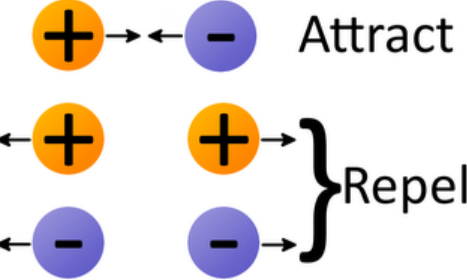
\includegraphics[width=0.75\linewidth]{vescschr.png}
            \end{figure}
        \end{alertblock}
    \end{columns}
\end{frame}

\begin{frame}
    \frametitle{Coulomb's Law - Key Properties}
    \begin{block}{Inverse Square Law}
        The electrostatic force is inversely proportional to the square of the distance between charges.
    \end{block}
    
    \begin{block}{Force Magnitude}
        \begin{itemize}
            \item Proportional to each charge magnitude
            \item Inversely proportional to distance squared
        \end{itemize}
    \end{block}
    
    \begin{block}{Force Direction}
        \begin{itemize}
            \item If $F < 0$ (negative result): attractive force
            \item If $F > 0$ (positive result): repulsive force
            \item Like charges repel, unlike charges attract
        \end{itemize}
    \end{block}
\end{frame}

\begin{frame}
    \frametitle{Electric Field}
    \begin{columns}
        \column{0.6\textwidth}
        \begin{block}{Definition}
            The electric field defines the force per unit charge in the space around a charge distribution.
        \end{block}
        
        \begin{block}{Mathematical Form}
            \begin{equation}
                \vec{E} = \frac{\vec{F}}{q}
            \end{equation}
            
            For a point charge or uniform sphere:
            \begin{equation}
                E = k\frac{q}{r^2}
            \end{equation}
        \end{block}
        
        \column{0.4\textwidth}
        \begin{alertblock}{ }
            \begin{figure}
                \centering
                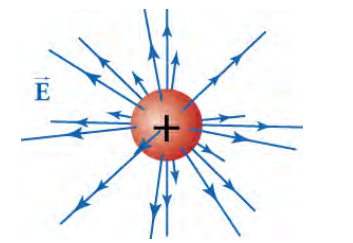
\includegraphics[width=0.75\linewidth]{posefeild.png}
            \end{figure}
        \end{alertblock}
    \end{columns}
\end{frame}

\begin{frame}
    \frametitle{Electric Field Properties}
    \begin{block}{Electric Field Lines}
        \begin{itemize}
            \item Electric field lines never cross each other
            \item More force is applied in regions with many field lines
            \item Field lines start at positive charges and point away
            \item Field lines end at negative charges and point toward them
        \end{itemize}
    \end{block}
    
    \begin{columns}
        \column{0.5\textwidth}
        \begin{alertblock}{  1}
            \begin{figure}
                \centering
                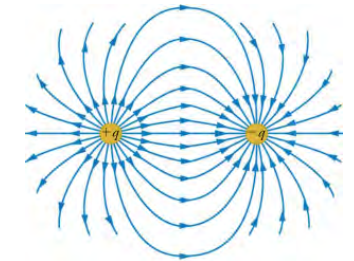
\includegraphics[width=1\linewidth]{opppfeldlins.png}
            \end{figure}
        \end{alertblock}
        
        \column{0.5\textwidth}
        \begin{alertblock}{  2}
            \begin{figure}
                \centering
                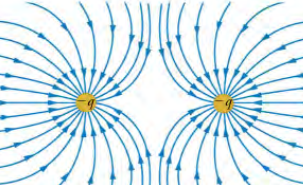
\includegraphics[width=1\linewidth]{lkfldlns.png}
            \end{figure}
        \end{alertblock}
    \end{columns}
\end{frame}

\begin{frame}
    \frametitle{Electric Potential}
    \begin{columns}
        \column{0.6\textwidth}
        \begin{block}{Electric Potential Energy}
            Similar to gravitational potential energy: the potential that charges have to do work by virtue of their positions relative to each other.
        \end{block}
        
        \begin{block}{Electric Potential}
            Electric potential is the electric potential energy per unit charge:
            \begin{equation}
                V = \frac{U}{q}
            \end{equation}
            
            For a point charge:
            \begin{equation}
                V = k\frac{q}{r}
            \end{equation}
        \end{block}
        
        \column{0.4\textwidth}
        \begin{alertblock}{ }
            \begin{figure}
                \centering
                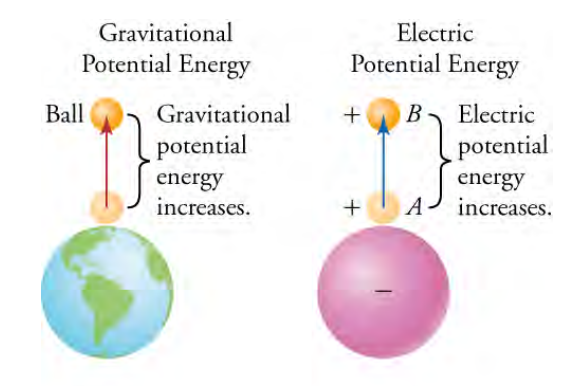
\includegraphics[width=1\linewidth]{ptnla.png}
            \end{figure}
        \end{alertblock}
    \end{columns}
\end{frame}

\begin{frame}
    \frametitle{Electric Potential - Key Properties}
    \begin{block}{Measurement}
        \begin{itemize}
            \item Potential is always measured between two points
            \item One point may be at infinity (reference point)
            \item Measured in volts (V)
        \end{itemize}
    \end{block}
    
    \begin{block}{Charge Movement}
        \begin{itemize}
            \item Positive charges move from high potential to low potential
            \item Negative charges move from low potential to high potential
            \item Charges move spontaneously to minimize potential energy
        \end{itemize}
    \end{block}
    
    \begin{block}{Relationship to Electric Field}
        \begin{equation}
            \vec{E} = -\nabla V
        \end{equation}
        The electric field points in the direction of decreasing potential.
    \end{block}
\end{frame}

\section{Capacitors and Dielectrics}

\begin{frame}
    \frametitle{Capacitors}
    \begin{columns}
        \column{0.6\textwidth}
        \begin{block}{Definition}
            A capacitor is a device that stores electric charge and energy in an electric field.
        \end{block}
        
        \begin{block}{Capacitance}
            Capacitance is the ratio of charge to voltage:
            \begin{equation}
                C = \frac{Q}{V}
            \end{equation}
            
            For a parallel plate capacitor:
            \begin{equation}
                C = \varepsilon_0 \frac{A}{d}
            \end{equation}
            where $A$ is plate area and $d$ is separation distance.
        \end{block}
        
        \column{0.4\textwidth}
        \begin{alertblock}{ }
            \begin{figure}
                \centering
                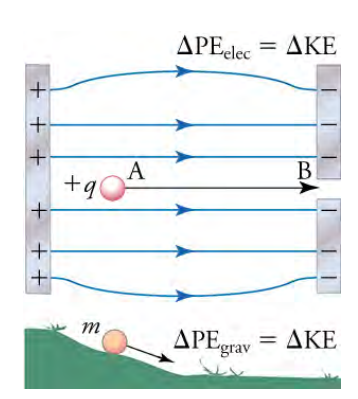
\includegraphics[width=1\linewidth]{earthcap.png}
            \end{figure}
        \end{alertblock}
    \end{columns}
\end{frame}

\begin{frame}
    \frametitle{Capacitors - Key Properties}
    \begin{block}{Capacitance Properties}
        \begin{itemize}
            \item Depends only on geometry and materials
            \item Does not depend on voltage across the capacitor
            \item Measured in farads (F)
        \end{itemize}
    \end{block}
    
    \begin{block}{Energy Storage}
        Capacitors store energy in the electric field between plates:
        \begin{equation}
            U = \frac{1}{2}CV^2 = \frac{1}{2}\frac{Q^2}{C} = \frac{1}{2}QV
        \end{equation}
    \end{block}
    
    \begin{block}{Electric Field in a Capacitor}
        \begin{equation}
            E = \frac{V}{d}
        \end{equation}
        where $d$ is the separation between plates.
    \end{block}
\end{frame}

\begin{frame}
    \frametitle{Dielectrics}
    \begin{columns}
        \column{0.6\textwidth}
        \begin{block}{Definition}
            A dielectric material is an insulator that becomes polarized in an electric field.
        \end{block}
        
        \begin{block}{Effect on Capacitance}
            Inserting a dielectric between capacitor plates increases capacitance:
            \begin{equation}
                C = \kappa \varepsilon_0 \frac{A}{d}
            \end{equation}
            where $\kappa$ is the dielectric constant (relative permittivity).
        \end{block}
        
        \column{0.4\textwidth}
        \begin{alertblock}{ }
           \begin{figure}
               \centering
               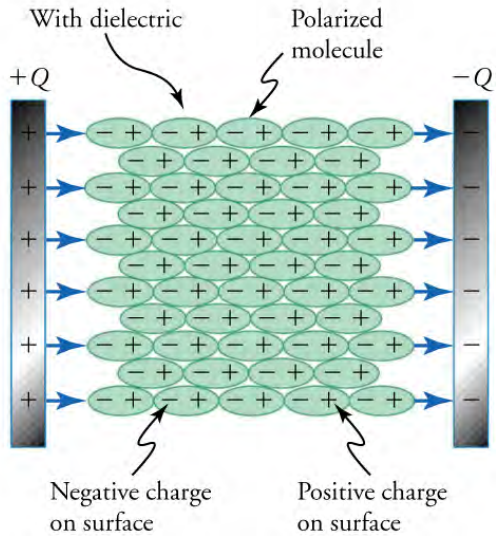
\includegraphics[width=1\linewidth]{dialecap.png}
           \end{figure}
        \end{alertblock}
    \end{columns}
\end{frame}

\section{Electric Circuits}

\begin{frame}
    \frametitle{Introduction to Electric Current}
    \begin{columns}
        \column{0.6\textwidth}
        \begin{itemize}
            \item \textbf{Direct Current (DC)}: Constant over time
            \item \textbf{Alternating Current (AC)}: Alternates smoothly back and forth over time
            \item \textbf{Electrical Resistance}: Causes materials to extract work from current flowing through them
        \end{itemize}
        
        \column{0.4\textwidth}
        \begin{alertblock}{ }
            \begin{figure}
                \centering
                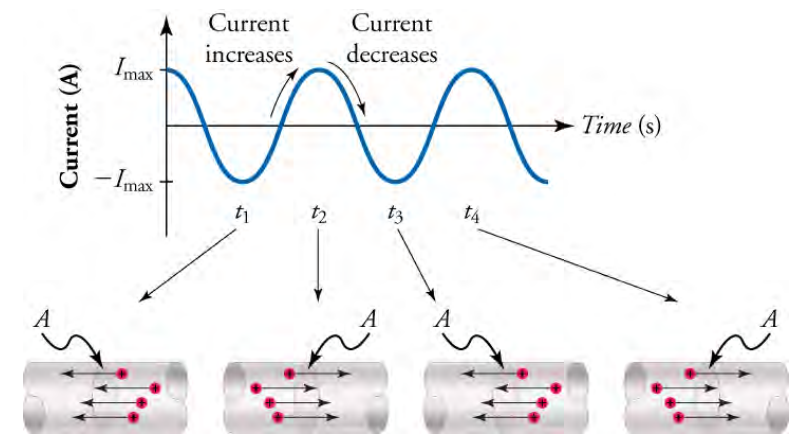
\includegraphics[width=1\linewidth]{ACDCCOM.png}
            \end{figure}
        \end{alertblock}
    \end{columns}
\end{frame}
\begin{frame}{}
\begin{figure}
                \centering
                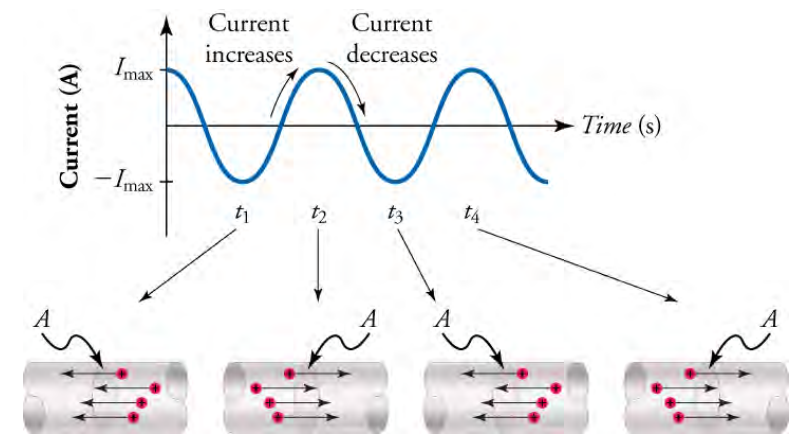
\includegraphics[width=1\linewidth]{ACDCCOM.png}
            \end{figure}    
\end{frame}
\begin{frame}
    \frametitle{Ohm's Law}
    \begin{columns}
        \column{0.6\textwidth}
        \begin{block}{Definition}
            In ohmic materials, voltage drop along a path is proportional to the current that runs through the path.
        \end{block}
        
        \begin{block}{Mathematical Form}
            \begin{equation}
                V = IR
            \end{equation}
            where:
            \begin{itemize}
                \item $V$ = voltage (volts, V)
                \item $I$ = current (amperes, A)
                \item $R$ = resistance (ohms, $\Omega$)
            \end{itemize}
        \end{block}
        
        \column{0.4\textwidth}
        \begin{alertblock}{ }
            \begin{figure}
                \centering
                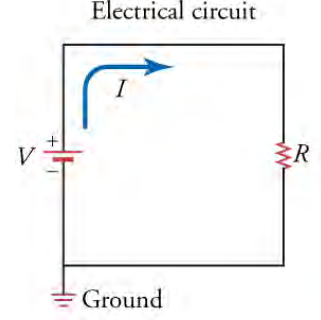
\includegraphics[width=1\linewidth]{simpcirc.png}
            \end{figure}
        \end{alertblock}
    \end{columns}
\end{frame}

\begin{frame}
    \frametitle{Series Circuits}
    \begin{columns}
        \column{0.6\textwidth}
        \begin{block}{Definition}
            Resistors in series are connected head to tail, with the same current flowing through each resistor.
        \end{block}
        
        \begin{block}{Key Properties}
            \begin{itemize}
                \item The same current flows through all resistors
                \item Voltage drops across each resistor can be different
                \item Voltage is the same at every point in a given wire
            \end{itemize}
        \end{block}
        
        \column{0.4\textwidth}
        \begin{alertblock}{ }
           \begin{figure}
               \centering
               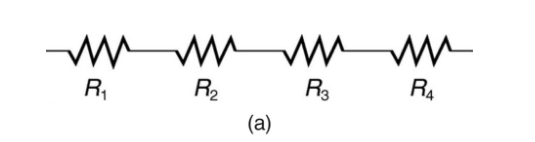
\includegraphics[width=1\linewidth]{serres.png}
           \end{figure}
        \end{alertblock}
    \end{columns}
\end{frame}

\begin{frame}
    \frametitle{Equivalent Resistance in Series}
    \begin{block}{Formula}
        For resistors in series, the total resistance is the sum of the individual resistances:
        \begin{equation}
            R_{\text{total}} = R_1 + R_2 + R_3 + \ldots + R_n
        \end{equation}
    \end{block}
    
    \begin{block}{Voltage Drops}
        The voltage drops across each resistor follow Ohm's law:
        \begin{equation}
            V_1 = IR_1, \quad V_2 = IR_2, \quad \ldots
        \end{equation}
        
        The total voltage across the circuit is the sum of the individual voltage drops:
        \begin{equation}
            V_{\text{total}} = V_1 + V_2 + V_3 + \ldots + V_n
        \end{equation}
    \end{block}
\end{frame}

\begin{frame}
    \frametitle{Parallel Circuits}
    \begin{columns}
        \column{0.6\textwidth}
        \begin{block}{Definition}
            Resistors in parallel are connected across the same two points in a circuit.
        \end{block}
        
        \begin{block}{Key Properties}
            \begin{itemize}
                \item Same voltage drop occurs across all resistors
                \item Current through each resistor can differ
                \item More paths for current means lower equivalent resistance
            \end{itemize}
        \end{block}
        
        \column{0.4\textwidth}
        \begin{alertblock}{ }
           \begin{figure}
               \centering
               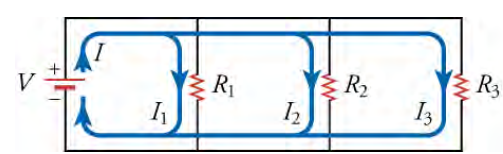
\includegraphics[width=1\linewidth]{resparr.png}
           \end{figure}
        \end{alertblock}
    \end{columns}
\end{frame}

\begin{frame}
    \frametitle{Equivalent Resistance in Parallel}
    \begin{block}{Formula}
        For resistors in parallel, the reciprocal of the total resistance equals the sum of the reciprocals of the individual resistances:
        \begin{equation}
            \frac{1}{R_{\text{total}}} = \frac{1}{R_1} + \frac{1}{R_2} + \frac{1}{R_3} + \ldots + \frac{1}{R_n}
        \end{equation}
    \end{block}
    
   
    \begin{block}{Important Note}
        The equivalent resistance of parallel resistors is always less than the smallest individual resistance.
    \end{block}
\end{frame}

\begin{frame}
    \frametitle{Electric Power}
    \begin{block}{Definition}
        Electric power is the rate at which electrical energy is converted to other forms of energy (heat, light, mechanical work, etc.).
    \end{block}
    
    \begin{block}{Key Concept}
        Electric power is dissipated in the resistances of a circuit. Capacitors do not dissipate electric power.
    \end{block}
    
    \begin{block}{Power Formula}
        Electric power is proportional to voltage and current:
        \begin{equation}
            P = VI
        \end{equation}
        where:
        \begin{itemize}
            \item $P$ = power (watts, W)
            \item $V$ = voltage (volts, V)
            \item $I$ = current (amperes, A)
        \end{itemize}
    \end{block}
\end{frame}

\begin{frame}
    \frametitle{Power Calculations}
    \begin{block}{Using Ohm's Law}
        Substituting $V = IR$ into $P = VI$:
        \begin{equation}
            P = VI = I(IR) = I^2R
        \end{equation}
        
        Alternatively, substituting $I = \frac{V}{R}$ into $P = VI$:
        \begin{equation}
            P = VI = V\left(\frac{V}{R}\right) = \frac{V^2}{R}
        \end{equation}
    \end{block}
    
    \begin{block}{Three Forms of Power Equation}
        \begin{equation}
            P = VI \quad \text{or} \quad P = I^2R \quad \text{or} \quad P = \frac{V^2}{R}
        \end{equation}
    \end{block}
\end{frame}

\section{Important Equations}

\begin{frame}
    \frametitle{Important Equations - Electrostatics}
    \begin{block}{Coulomb's Law}
        \begin{equation}
            F = k\frac{q_1 q_2}{r^2}
        \end{equation}
    \end{block}
    
    \begin{block}{Electric Field}
        \begin{equation}
            E = k\frac{q}{r^2} \quad \text{and} \quad \vec{E} = \frac{\vec{F}}{q}
        \end{equation}
    \end{block}
    
    \begin{block}{Electric Potential}
        \begin{equation}
            V = k\frac{q}{r} \quad \text{and} \quad V = \frac{U}{q}
        \end{equation}
    \end{block}
    
    \begin{block}{Capacitance}
        \begin{equation}
            C = \frac{Q}{V} \quad \text{and} \quad C = \kappa\varepsilon_0\frac{A}{d}
        \end{equation}
    \end{block}
\end{frame}

\begin{frame}
    \frametitle{Important Equations - Circuits}
    \begin{block}{Ohm's Law}
        \begin{equation}
            V = IR
        \end{equation}
    \end{block}
    
    \begin{block}{Series Circuits}
        \begin{equation}
            R_{\text{total}} = R_1 + R_2 + R_3 + \ldots + R_n
        \end{equation}
    \end{block}
    
    \begin{block}{Parallel Circuits}
        \begin{equation}
            \frac{1}{R_{\text{total}}} = \frac{1}{R_1} + \frac{1}{R_2} + \frac{1}{R_3} + \ldots + \frac{1}{R_n}
        \end{equation}
    \end{block}
    
    \begin{block}{Electric Power}
        \begin{equation}
            P = VI = I^2R = \frac{V^2}{R}
        \end{equation}
    \end{block}
\end{frame}

\section{Examples}

\begin{frame}
    \frametitle{I Do: Coulomb's Law Application}
    \begin{block}{Problem}
        Two point charges, $q_1 = 3 \,\mu\text{C}$ and $q_2 = -2 \,\mu\text{C}$, are separated by a distance of 15 cm. Calculate the electrostatic force between them.
    \end{block}
    \end{frame}

\begin{frame}
    \begin{block}{Solution}
        Using Coulomb's law: $F = k\frac{q_1 q_2}{r^2}$
        
        Given:
        \begin{itemize}
            \item $q_1 = 3 \times 10^{-6} \,\text{C}$
            \item $q_2 = -2 \times 10^{-6} \,\text{C}$
            \item $r = 0.15 \,\text{m}$
            \item $k = 8.99 \times 10^9 \,\text{N}\cdot\text{m}^2/\text{C}^2$
        \end{itemize}
        
        Substituting:
        \begin{align}
            F &= (8.99 \times 10^9) \frac{(3 \times 10^{-6})(-2 \times 10^{-6})}{(0.15)^2} \\
            F &= (8.99 \times 10^9) \frac{-6 \times 10^{-12}}{0.0225} \\
            F &= -2.4 \,\text{N}
        \end{align}
        
        The negative sign indicates an attractive force.
    \end{block}
\end{frame}

\begin{frame}
    \frametitle{We Do: Electric Potential Problem}
    \begin{block}{Problem}
        A point charge of $5 \,\mu\text{C}$ creates an electric potential. Calculate the electric potential at points 10 cm and 20 cm from the charge.
    \end{block}
    \end{frame}

\begin{frame}
    \begin{block}{Solution - Let's solve together}
        Using the formula for electric potential due to a point charge:
        \begin{equation}
            V = k\frac{q}{r}
        \end{equation}
        
        At $r_1 = 10 \,\text{cm} = 0.1 \,\text{m}$:
        \begin{align}
            V_1 &= k\frac{q}{r_1} \\
            V_1 &= (8.99 \times 10^9) \frac{5 \times 10^{-6}}{0.1} \\
            V_1 &= ?
        \end{align}
        
        At $r_2 = 20 \,\text{cm} = 0.2 \,\text{m}$:
        \begin{align}
            V_2 &= k\frac{q}{r_2} \\
            V_2 &= (8.99 \times 10^9) \frac{5 \times 10^{-6}}{0.2} = ?
        \end{align}
    \end{block}
\end{frame}

\begin{frame}
    \frametitle{I Do: Series Circuit Analysis}
    \begin{block}{Problem}
        Three resistors of 2 $\Omega$, 4 $\Omega$, and 6 $\Omega$ are connected in series with a 12 V battery. Calculate:
        \begin{enumerate}
            \item The total resistance
            \item The current in the circuit
            \item The voltage drop across each resistor
        \end{enumerate}
    \end{block}
    \end{frame}

\begin{frame}
    \begin{block}{Solution}
        \begin{enumerate}
            \item Total resistance:
            \begin{align}
                R_{\text{total}} &= R_1 + R_2 + R_3 \\
                R_{\text{total}} &= 2\,\Omega + 4\,\Omega + 6\,\Omega = 12\,\Omega
            \end{align}
            
            \item Current (using Ohm's law):
            \begin{align}
                I &= \frac{V}{R_{\text{total}}} = \frac{12\,\text{V}}{12\,\Omega} = 1\,\text{A}
            \end{align}
            
            \item Voltage drops:
            \begin{align}
                V_1 &= IR_1 = (1\,\text{A})(2\,\Omega) = 2\,\text{V} \\
                V_2 &= IR_2 = (1\,\text{A})(4\,\Omega) = 4\,\text{V} \\
                V_3 &= IR_3 = (1\,\text{A})(6\,\Omega) = 6\,\text{V}
            \end{align}
            
            Note that $V_1 + V_2 + V_3 = 2\,\text{V} + 4\,\text{V} + 6\,\text{V} = 12\,\text{V}$, which equals the battery voltage.
        \end{enumerate}
    \end{block}
\end{frame}

\begin{frame}
    \frametitle{We Do: Parallel Circuit Problem}
    \begin{block}{Problem}
        Three resistors of 3 $\Omega$, 6 $\Omega$, and 9 $\Omega$ are connected in parallel. Calculate:
        \begin{enumerate}
            \item The equivalent resistance
            \item If this circuit is connected to a 12 V battery, find the total current drawn from the battery
        \end{enumerate}
    \end{block}
    \end{frame}

\begin{frame}
    \begin{block}{Solution - Let's solve together}
        \begin{enumerate}
            \item Equivalent resistance:
            \begin{align}
                \frac{1}{R_{\text{eq}}} &= \frac{1}{R_1} + \frac{1}{R_2} + \frac{1}{R_3} \\
                \frac{1}{R_{\text{eq}}} &= \frac{1}{3\,\Omega} + \frac{1}{6\,\Omega} + \frac{1}{9\,\Omega} \\
                \frac{1}{R_{\text{eq}}} &= \frac{3 + 1.5 + 1}{9\,\Omega} = \frac{5.5}{9\,\Omega} \\
                R_{\text{eq}} &= \frac{9\,\Omega}{5.5} = ? \,\Omega
            \end{align}
            
            \item Total current:
            \begin{align}
                I_{\text{total}} &= \frac{V}{R_{\text{eq}}} = \frac{12\,\text{V}}{R_{\text{eq}}} = ?
            \end{align}
        \end{enumerate}
    \end{block}
\end{frame}

\begin{frame}
    \frametitle{You Do: Combined Problem}
    \begin{block}{Problem}
        A 12 V battery is connected to a parallel plate capacitor with a separation of 2 mm. The capacitor has a capacitance of 5 $\mu$F.
        \begin{enumerate}
            \item Calculate the electric field between the plates
            \item Calculate the electric energy stored in the capacitor
            \item If a dielectric with $\kappa = 4$ is inserted between the plates, what is the new capacitance?
            \item Calculate the capacitor charge before and after inserting the dielectric
        \end{enumerate}
    \end{block}
    
    \begin{alertblock}{Hints}
        \begin{itemize}
            \item Electric field in a parallel plate capacitor: $E = \frac{V}{d}$
            \item Energy stored in a capacitor: $U = \frac{1}{2}CV^2$
            \item Capacitance with dielectric: $C = \kappa C_0$
            \item Charge on a capacitor: $Q = CV$
        \end{itemize}
    \end{alertblock}
\end{frame}

\section{Summary}

\begin{frame}
    \frametitle{Summary - Electrostatics}
    \begin{columns}
        \column{0.5\textwidth}
        \begin{block}{Coulomb's Law}
            \begin{itemize}
                \item Inverse square law
                \item $F = k\frac{q_1 q_2}{r^2}$
                \item Like charges repel, unlike attract
            \end{itemize}
        \end{block}
        
        \begin{block}{Electric Field}
            \begin{itemize}
                \item Force per unit charge
                \item $E = k\frac{q}{r^2}$
                \item Field lines show direction of force
            \end{itemize}
        \end{block}
        
        \column{0.5\textwidth}
        \begin{block}{Electric Potential}
            \begin{itemize}
                \item Potential energy per unit charge
                \item $V = k\frac{q}{r}$
                \item Charges move to minimize potential energy
            \end{itemize}
        \end{block}
        
        \begin{block}{Capacitors}
            \begin{itemize}
                \item Store energy in electric field
                \item $C = \frac{Q}{V}$
                \item Dielectrics increase capacitance
            \end{itemize}
        \end{block}
    \end{columns}
\end{frame}

\begin{frame}
    \frametitle{Summary - Electric Circuits}
    \begin{columns}
        \column{0.5\textwidth}
        \begin{block}{Ohm's Law}
            \begin{itemize}
                \item $V = IR$
                \item Direct vs. alternating current
                \item Ohmic materials
            \end{itemize}
        \end{block}
        
        \begin{block}{Series Circuits}
            \begin{itemize}
                \item Same current through all resistors
                \item $R_{\text{total}} = R_1 + R_2 + \ldots$
                \item Voltage drops can differ
            \end{itemize}
        \end{block}
        
        \column{0.5\textwidth}
        \begin{block}{Parallel Circuits}
            \begin{itemize}
                \item Same voltage across all resistors
                \item $\frac{1}{R_{\text{total}}} = \frac{1}{R_1} + \frac{1}{R_2} + \ldots$
                \item Currents can differ
            \end{itemize}
        \end{block}
        
        \begin{block}{Electric Power}
            \begin{itemize}
                \item $P = VI = I^2R = \frac{V^2}{R}$
                \item Power dissipated in resistances
                \item Measured in watts (W)
            \end{itemize}
        \end{block}
    \end{columns}
\end{frame}



\begin{frame}
    \frametitle{Thank You!}
    \begin{center}
        \Large Any questions?
        
        \vspace{1cm}
        
        \normalsize For additional practice problems, refer to your textbook Chapters 18-19
    \end{center}
\end{frame}

\end{document}